\documentclass[letterpaper]{article}
\usepackage[submission]{aaai2027}
% Fonts are managed by the unmodified official AAAI-27 style.
\usepackage[hyphens]{url}
\usepackage{graphicx}
\urlstyle{rm}
\def\UrlFont{\rm}
\usepackage{natbib}
\usepackage{caption}
\frenchspacing
\usepackage{amsmath,amssymb,booktabs,array}
\pdfinfo{/TemplateVersion (2027.1)}
\setcounter{secnumdepth}{0}
\newtheorem{proposition}{Proposition}
\newenvironment{proof}{\par\noindent\textit{Proof.}\ }{\hfill$\square$\par}
\newcommand{\enc}{\Phi}
\title{Compositional Narrative Planning through Source-Preserving Domain Fusion}
\author{Anonymous Authors}
\affiliations{}
\begin{document}
\maketitle
\begin{abstract}
We combine existing narrative planning domains so that a planner can build a story using events from more than one domain. For example, acquiring a key in one model could enable entry to an archive in another. We adapt UniDomain's approach of selecting and combining planning domains to models learned from stories. Our method connects predicates that describe the same fact, records which characters and objects are shared, and keeps each source action's conditions and effects. Distinct events remain separate; compatible actions can be combined under a restricted rule that preserves alternative conditions. We give sufficient conditions under which original plans remain executable after translation. One completed experimental repeat, resumed after interruption, covers 300 groups from 60 previously admitted learned domains. All 499 available plan translations validate, covering 55.44\% of registered cases and reusing 33 original plans. A separate posthoc diagnostic covers 70 tasks in 37 distinct constructed worlds. Full confirms 50 cross-source plans, with ten action-origin verdicts unknown; predicate sharing alone confirms 56. A separately authored 11-step case uses four sources through a cross-source link and independent goal branches. These results support conditional preservation and event composition, without establishing four-source causal chains or story quality.
\end{abstract}

\section{Introduction}
Narrative planning constructs story events from a model of what characters can do and how their actions change the world. The available actions limit the stories a planner can produce, and building this knowledge requires substantial effort~\cite{hayton2020acquisition,cheng2025verbnet}. We study how to reuse existing narrative planning domains together: can an event from one model enable an event from another, while the original actions remain usable?

In Figure~\ref{fig:motivation}, model A describes obtaining an object; model B describes opening an archive and retrieving evidence. Combining them lets Mira receive a key using A and unlock the archive using B. Neither model alone describes the whole sequence. Buying or stealing the key could offer other routes with different consequences. Reusing these events could extend the plots available to an author. Whether the resulting stories are better also depends on coherence, character motivation, and reader interest~\cite{rivera2024story}.

\begin{figure*}[t]
\centering
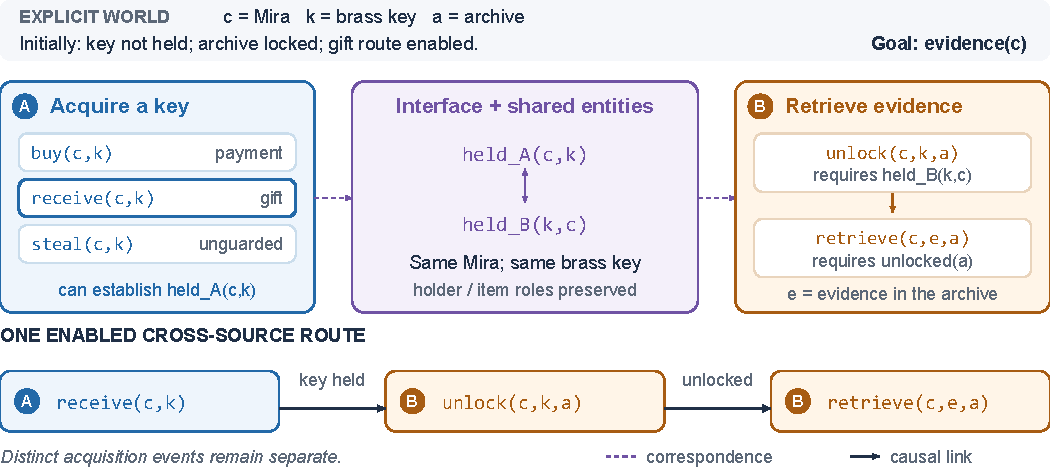
\includegraphics[width=\textwidth]{figures_2026_11_03_v1/figure1_causal_composition.pdf}
\caption{An illustrative example, not experimental data. Model A lets Mira obtain a key; model B lets her use it to enter an archive. Their possession predicates must refer to the same Mira and key, with the correct argument order. Buying, receiving, and stealing retain their own rules.}
\label{fig:motivation}
\end{figure*}

Our starting point is UniDomain, which learns planning domains from robot demonstrations, retrieves relevant domains, and combines them before planning~\cite{ye2025unidomain}. We adapt this approach to existing models learned from stories, using them as the input for new combinations of events.

Story models differ in ways that matter when combining them. A purchase and a gift may both give Mira a key, but have different conditions and narrative meanings. Two possession predicates may list the person and object in opposite orders. Models may also describe different characters and worlds; matching a type name does not make two objects identical. These issues are not unique to narratives, but they determine whether the combined events make sense.

Our method connects predicates judged to describe the same fact, records shared characters and objects, and retains each action's conditions and effects. Distinct events remain separate. Compatible actions can optionally be combined when their effects agree, keeping their conditions as alternatives. The output is a reusable planning domain, saved with its mappings before search. Sharing facts lets events from different sources interact; combining actions is a separate step for reducing duplication.

\paragraph{Contributions.}
(1) We define the required mappings between narrative models. (2) We give a domain construction and sufficient conditions for retaining original plans. (3) We separately evaluate plan preservation, combinations of events across sources, and action merging.

The evaluation uses 300 groups from 60 previously admitted learned domains. All 499 available translations of original plans validate, though they reuse 33 plans and cover only 55.44\% of registered cases. A separate 70-task diagnostic confirms 50 cross-source Full plans, with ten origin-unknown; predicate sharing alone confirms 56. A distinct authored 11-step case uses all four sources. These results support the construction within the tested cases; semantic mappings, longer connected chains, and story quality require further evaluation.

\section{Background and Problem Definition}
\subsection{Narrative Planning Models}
A planning \emph{domain} describes reusable actions and rules. Predicates represent facts, such as a character holding a key. Each action specifies its participants, required conditions, and effects. A planning \emph{problem} supplies objects, an initial state, and a goal. The planner searches for an action sequence reaching that goal. Narrative models may also specify actors and their intentions~\cite{riedl2010narrative}. Our experiments retain these annotations and use the narrative planner's explanation checks; the preservation argument below concerns Boolean state changes.

\subsection{From UniDomain to Narrative Domains}
UniDomain has three stages~\cite{ye2025unidomain}. First, it learns small domains from robot demonstrations, typically of one operation. Second, it retrieves relevant domains using language-model suggestions and embedding similarity, then combines them pairwise in a binary tree. A language model checks predicates and actions for equivalence; the described action merge collects their preconditions and effects. Third, it constructs a problem from a task instruction and scene image and runs a planner.

We retain selection and fusion before planning, with three changes for narrative reuse. First, we start from existing story models, using supplied groups or the dependency-based selector below. Selection keeps whole domains. A language model judges candidate mappings, and a fixed compiler applies accepted mappings to the action rules. Second, we specify shared facts and objects separately. In Figure~\ref{fig:motivation}, \texttt{held\_A(c,k)} and \texttt{held\_B(k,c)} describe the same fact only with the correct argument order and the same character and key. We also record which objects belong to each source type. This prevents a rule about ``every guard'' in one source from unexpectedly including another source's guards.

Third, sharing a fact does not require combining the events that establish it. Buying and receiving can share possession while keeping different requirements. Actions remain separate unless they are judged compatible and their mapped effects pass an equality check. A combined action accepts either source's full conditions, including its object restrictions. In the learned-domain adapter, the acting roles must also agree. This preserves alternative ways to perform a compatible action without equating all events that have the same outcome.

\subsection{Task Definition}
\paragraph{Inputs and output.}
Let $\mathcal D=\{D_1,\ldots,D_m\}$ be finite typed domains with Boolean predicates, parameterized instantaneous actions, and source constants. From selected domains and accepted mappings, we construct $D^*$ and record how source predicates, actions, and constants map into it. The output remains parameterized for use with multiple problems, and all construction decisions are fixed before search.

Each request supplies objects, their source type memberships, an explicit initial state $I$, and optionally a goal $G$. Facts absent from $I$ are false. Missing $I$ requires clarification before construction or search; an explicitly empty state is valid. Shared objects must be declared, and original source facts are never automatically added. Without a goal, the system generates reachable outcomes as described below.

\paragraph{Two requirements.}
First, original plans should remain executable after translation under the assumptions in the preservation proposition. Each original problem is checked separately. Second, an event from one source should be able to establish a fact needed by another source's event toward the goal. This requires a declared common world. We evaluate the two requirements separately; neither guarantees correct semantic mappings or interesting stories.

\paragraph{Mapping assumptions.}
For source $i$, object renaming $\eta_i$ is injective, and source constants remain distinct. Each predicate $p$ maps to a target $\mu_i(p)$ with a bijection $\pi_{i,p}$ over argument positions. Different predicates within one source cannot share a target; predicates from different sources may do so. An accepted mapping, called a \emph{predicate interface}, records source hashes, supporting evidence, the decision basis, argument order, and assumed argument types. Structural validity does not establish semantic correctness.

\paragraph{Supported language.}
The implementation supports conjunction, disjunction, negation, equality, existential and universal conditions, and conditional and universal effects, within the combinations accepted by the independent parser. UP 1.3.0 currently rejects nested universal effects. Numeric fluents, temporal actions, derived predicates, and partial-observation semantics are outside the supported language. Unsupported constructs are rejected rather than removed.

\section{Constructing the Combined Domain}
We build one reusable domain from the selected source models. The construction has four steps: select domains, match predicates and their arguments, specify which objects can be shared, and translate the actions. Compatible actions may then be combined. Figure~\ref{fig:pipeline} shows this process and the two ways we check its output.

\begin{figure*}[t]
\centering
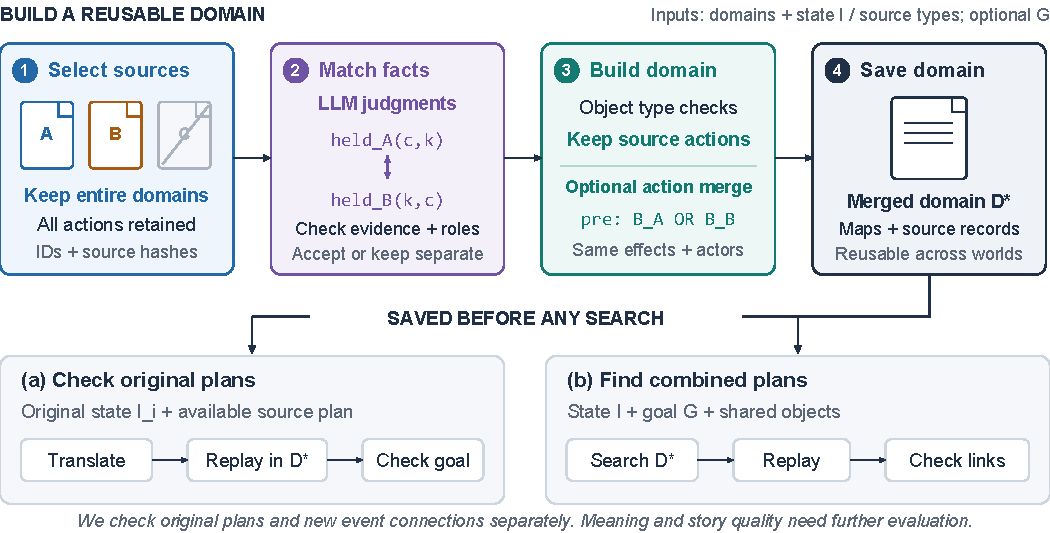
\includegraphics[width=\textwidth]{figures_2026_11_03_readability_v1/figure2_construction_and_evaluation.pdf}
\caption{Construction and evaluation. All actions from selected sources are retained with their object restrictions. Accepted predicates are connected; compatible actions with equal effects may be combined. The saved domain $D^*$ supports two checks: translating original plans and finding plans that connect events across sources. Neither check assesses story quality.}
\label{fig:pipeline}
\end{figure*}


\subsection{Select Source Domains}
The user can supply a group of domains, as in our main experiment. When selection is driven by a goal, we start from its predicates and work backward: an action that can produce a needed fact introduces the predicates in its conditions as further dependencies. We keep every action from each selected domain. We also retain sources named in the request and all sources participating in an accepted shared-predicate group.

This dependency check ignores argument bindings and whether a condition is positive or negative, so it can retain more sources than necessary. For a request without a goal, it keeps all sources unless an explicit group is supplied. The supplement gives a separate optional reduction that can remove irrelevant sources for a fixed world.

\subsection{Match Facts Across Domains}
Two domains can describe the same relation with different predicate names or argument orders. In the key example, one may write \texttt{held\_A(person,key)} and the other \texttt{held\_B(key,person)}. We must match both the possession relation and the person/key positions before one model's action can enable the other's.

For the learned-domain study, a language model judges candidate pairs using their declarations and action contexts. Each proposed match records the meaning, argument roles, confidence, and supporting source evidence. The system checks the response and the proposed argument mapping before accepting it. A group of matches must agree for every pair and give a consistent argument order around any cycle. Rejected, invalid, or unavailable judgments leave the predicates separate. These checks make the mappings consistent and inspectable; they do not independently establish that the model's judgment is correct.

Using the notation from the problem definition, translation of a source atom is
\begin{equation}
\begin{split}
\enc_i\bigl(p(x_1,\ldots,x_k)\bigr)
={}&\mu_i(p)\bigl(\eta_i(x_{\pi_{i,p}(1)}),\ldots,\\
&\hspace{2em}\eta_i(x_{\pi_{i,p}(k)})\bigr).
\end{split}
\end{equation}
Here $\mu_i$ gives the shared predicate name, $\pi_{i,p}$ puts arguments in the agreed order, and $\eta_i$ renames objects. We apply the same translation to initial facts, goals, conditions, and effects, including their negations. Missing argument positions, invalid permutations, stale source files, and missing argument-type mappings are rejected. A direction-sensitive test in the supplement shows why reversing two roles can break a plan.

\subsection{Specify Shared Objects and Retain Types}
Matching predicates does not identify their objects. A request must explicitly state when two sources refer to the same character or item. It must also state the source types to which that object belongs. A shared key can then be used by actions from both sources. A match between type names alone neither identifies source constants nor grants an object an additional type membership.

Keeping source types matters for conditions about all objects of a type. Suppose a rule requires every guard in source A to be ready. Adding source B should not make the rule also require B's guards to be ready. We therefore record each source type using a predicate $M_{i,T}(x)$: object $x$ belongs to type $T$ in source $i$. Declared objects and constants receive memberships for their types and ancestor types. Actions cannot change these memberships. They are bookkeeping facts, recorded separately from the story's initial facts.

An action parameter can be bound only to objects with its original source membership. Quantified conditions use the same restriction:
\begin{equation}
\begin{aligned}
\enc_i(\forall x{:}T\;\varphi)
&=\forall x\;\bigl(M_{i,T}(x)\Rightarrow\enc_i(\varphi)\bigr),\\
\enc_i(\exists x{:}T\;\varphi)
&=\exists x\;\bigl(M_{i,T}(x)\land\enc_i(\varphi)\bigr),
\end{aligned}
\end{equation}
Thus ``all $T$'' checks only the original $T$ objects, and ``some $T$'' requires one of those objects. Universal effects are restricted in the same way. Conditional-effect tests are retained, as are additions, deletions, and negation. Before rewriting a quantified expression, the compiler gives bound variables fresh names so that a reused variable name cannot change which participant it refers to. Encoding types as predicates is an established representation technique; here it makes each source's object restrictions explicit.

\subsection{Retain Actions and Optionally Combine Them}
We translate each source action and keep it as a separate action by default. This lets buying, receiving, and stealing share possession without making them the same event. Each retains its own conditions and consequences. We call these separately retained actions \emph{source action variants}.

Combining actions is a separate, optional step. It requires a judgment that the events are compatible, a complete mapping of all parameters, and equality of the mapped effects. Parameters used only in conditions must also be mapped. Let $B_j(\bar x)$ be the full translated condition of action $a_j$, including the source type restrictions. If every action has the same additions $E^+$ and deletions $E^-$, the combined action is
\begin{equation}
a^*(\bar x)=\left\langle\bigvee_j B_j(\bar x),\ E^+,\ E^-\right\rangle.
\end{equation}
The OR means that satisfying either source's complete conditions is enough. For example, two compatible versions of a travel action may require different permissions; one need not require both permissions. The effects stay the same whichever alternative enables the action.

The implemented action-merging check supports a smaller language than the general translator: actions with unsupported quantifiers, conditional effects, function terms, or numeric updates remain separate. In the learned-domain adapter, acting roles must also agree, and problems retain their original intentions. A below-threshold or invalid semantic judgment also leaves actions separate.

Under the initial-state assumptions below, an executable source action satisfies its own alternative in the combined action. Equal effects give the same next source state. Repeating this argument preserves an original source plan. This gives a sufficient condition for retaining those plans. Whether combining actions reduces model size or search cost must be measured separately; shared predicates can already connect events without action merging.

\subsection{Save the Domain and Run the Planner}
Before search, we save the parameterized domain, source hashes, accepted mappings, and action origins. The planner then receives this fixed model and an explicitly supplied problem. Original source problems are translated separately for preservation checks. New combinations use a declared common world with its own objects, initial state, and goal.

The learned-domain experiments use Glaive, retaining actors and intentions. Returned plans must pass Glaive's explanation and goal checks and an independent check of action applicability and the goal. A timeout, no returned plan, or unsupported result keeps its own status. For requests without a goal, the generic implementation returns reachable noninitial states and plans in bounded breadth-first order; it does not rank their story quality. Search details are in the supplement.

\section{When Original Plans Remain Valid}
The construction is intended to keep original actions usable. The guarantee requires the translated problem to start with the same source facts and the same source objects, after renaming. This includes facts that are false: adding only the source's positive facts may be insufficient if another source assigns a different truth value to a shared fact.

Let $I_i$ be the original initial state and $J$ the target initial state. For every well-typed ground source atom $A$, we require
\[
J\models\enc_i(A)\quad\Longleftrightarrow\quad I_i\models A
\]
The following proposition states the remaining conditions precisely.

\begin{proposition}[Source-local trace preservation]
\label{prop:source-local}
Fix a finite source problem $P_i$ in the supported fragment. Assume that (i) $\eta_i$ and the source-local predicate map are injective; (ii) each argument map is a bijection; (iii) $M_{i,T}$ denotes exactly the image of the original source type extension, remains immutable, and guards all parameter and quantified occurrences; (iv) $J$ satisfies the initial-state premise above and the goal uses the same formula translation; and (v) each source action variant is retained with the stated capture-avoiding condition/effect translation, with no other added precondition or effect. Then every valid source-only trace in $P_i$ has a valid action-wise translation in the compiled domain, with the same truth values for mapped source atoms after each step. The statement is independent of whether the asserted cross-source correspondence has the intended narrative meaning.
\end{proposition}
\begin{proof}
First, translation preserves the truth of each source formula. Object and predicate injectivity preserve distinct atoms; the argument mapping keeps the prescribed argument order. Boolean operations and equality keep their meanings. Membership conditions make quantifiers range over exactly the original objects, and fresh bound-variable names preserve variable scope. Action parameters therefore have the same legal bindings. An action's conditions have the same truth value before translation and after it. Its effects make the same additions and deletions: conditional effects use the same tests, and universal effects cover the same objects. Hence one translated action gives the corresponding source state. Applying this argument to each action preserves the whole trace and the translated goal, assuming well-defined simultaneous effects in the valid source trace.
\end{proof}

\paragraph{Preservation and meaning.}
The proposition concerns plans using one source's actions in a matching initial state. A new plan that mixes sources needs additional semantic justification. For example, an incorrect possession match could leave every original plan executable while enabling an implausible combination. Preservation checks therefore test execution; independent judgments are needed to check the meanings of shared facts and objects. The sufficient conditions also remain subject to independent technical review.

\paragraph{Keep original worlds separate.}
Two original problems may disagree about a fact that becomes shared. If one says it is true and the other says it is false, no single initial state can preserve both values. We check each original problem separately and require an explicit initial state for new combinations. An optional audit can enumerate mapped source atoms and report conflicting truth values. Reaching its atom budget gives an unknown result; finding no conflict checks only initial-state compatibility. The audit never creates a pooled world or supplies missing initial facts.

\section{Evaluation}
We ask two questions. After combining domains, can we still execute the available original plans? Can we also find a plan in which an event from one source enables an event from another toward the goal? The first checks retention of existing behavior; the second checks new combinations. The archive example in Figure~\ref{fig:motivation} illustrates the idea and is not an experimental task.

\subsection{Data and Setup}
We use the \emph{GPT-4 revised} artifacts of \emph{There and Back Again}~\cite{kelly2023there}. The recorded collection has 192 sources: 40 in the legacy development split and 152 in its test split. Our existing parser/compiler checks admit 60 of the latter, comprising 32 TinyStories and 28 WritingPrompts domains. The other 92 remain documented exclusions. We do not repair the sources. We have already examined the admitted models during development, so their original test-split label does not make this an unseen-source evaluation.

Before model judgments or search, we fix 100 balanced sequences of source identifiers and take their first two, three, and four entries. This gives 100 groups per size, 300 groups in total, and 538 distinct source pairs. Selection uses identifiers rather than semantic scores or planning outcomes. Groups overlap, so their results are correlated. The supplement gives the exact balancing and sampling rules.

We compare four conditions. \emph{Native} plans with an original domain and problem. \emph{Union} puts selected domains together but keeps their predicates and actions separate. \emph{Predicate-only} shares accepted predicates and keeps the source actions separate. \emph{Full} uses the same predicate matches and also combines eligible actions with matching effects and acting roles. This comparison shows whether a result comes from sharing facts or from merging actions. All 900 combined domains and mappings are saved before main-experiment search.

GLM-5.3 Cloud judges candidate matches; acceptance requires confidence at least 0.9 and the evidence, argument, and consistency checks described above. Glaive search and replay each have a 15-second limit, a 4-GB Java limit, and one planner worker. We retain source actors and intentions and use a versioned runtime correcting false-disjunction substitution and empty-type grounding. The main search block has 60 Native calls and 1,800 merged-domain calls: two fixed original problems per group under three conditions. Each such problem activates only its own source, with no imported initial facts. Model options, candidate limits, runtime changes, and complete outcomes are in the supplement.

We report one completed run that was resumed after interruption. Five runs were registered; the second stopped at the service quota and the remaining runs are incomplete. This run retains the serial and ten-client request segments and their unsuccessful outcomes. It therefore supplies neither a five-run stability estimate nor a timing comparison.

\subsection{Checking Original Plans}
We first record what actually changed in the domains. Of 4,680 model judgments, 4,117 pass the required response checks, 561 are invalid, and two are unavailable. Passing these checks measures usable output, not semantic accuracy. Among the valid judgments, 206 propose compatibility. Predicate sharing occurs in 120 of the 300 groups and action merging in 19. The supplement reports the distinct pairs, repeated merge occurrences, and rejected outputs.

\begin{table}[t]
\centering
\caption{Do original plans still execute in Full? Each size has 100 domain groups. Pred./Act. count groups with predicate/action merges. Replayed gives passed/available plan checks; Unavailable counts missing validated reference plans.}
\label{tab:revised-preservation}
\begin{tabular}{rrrrr}
\toprule
$k$ & Pred. & Act. & Replayed & Unavailable\\
\midrule
2 & 15 & 0 & 111/111 & 89\\
3 & 42 & 7 & 165/165 & 135\\
4 & 63 & 12 & 223/223 & 177\\
Total & 120 & 19 & 499/499 & 401\\
\bottomrule
\end{tabular}
\end{table}

For each source in each group, we try to execute its validated Native plan in the merged domain using the original initial state and goal. Each source--group pair is one test case, giving $N=100(2+3+4)=900$ Full cases. If a validated Native plan exists, we translate and replay it. A pass requires Glaive goal achievement with no unexplained steps, plus an independent applicability and goal check. We report passed/available checks $V/A$ and coverage $A/N$ separately.

Every available Full check passes: $499/499$ (Table~\ref{tab:revised-preservation}). These checks reuse 33 distinct Native plans, of length 1--20, across merged domains. Native search returns 34 plans, of which 33 validate and one uses unsupported counterfactual steps; 16 searches return no plan and ten time out. As a result, 401 of the 900 cases have no validated reference plan. Preservation is 100\% among the tested cases, with 55.44\% evidence coverage. Union and Predicate-only have the same outcomes. The 1,497 passes across all three conditions repeatedly use these 33 plans.

The groups with actual merges also retain every available plan: $206/206$ checks in predicate-sharing groups, out of 408 cases, and $35/35$ in action-merging groups, out of 69 cases. Coverage of merged actions is narrower. The 19 merged actions replace 38 source-action alternatives. A Native plan is available for 19 alternatives, but only 11 are exercised by a merged step. Structural checks pass for all 19 merges, while untested alternatives remain uncovered.

We also run fresh searches on the 600 original problems in each merged condition. All three conditions have identical statuses: 341 returned plans, of which 332 validate and nine remain unknown; 160 no-plan returns and 99 timeouts. The unknowns reuse one source with unsupported counterfactual syntax. These searches check original problems, with only one source active. They do not test whether different sources can interact, and a no-plan return within the budget is not a proof of unsolvability.

\subsection{Combining Events from Different Sources}
We separately test the unchanged saved domains in explicit constructed worlds. After observing the accepted mappings, a restricted generator seeks a positive fact produced by one source's action and required by another's. It supports conjunctive conditions and no constant bindings. Objects, shared identities, memberships, initial facts, intentions, and goals are declared before search; no original problem facts are pooled.

Only 35 of 300 groups support this rule. Of the remainder, 180 have no accepted shared predicate, 83 lack a supported positive producer--consumer pair, and two lack a distinct positive goal effect. These are interface/generator coverage limits, not 265 established composition failures. The generator excludes 74 source actions with unsupported formulas and three with constant bindings; these action counts do not partition the group counts.

An earlier 18-task diagnostic selected one descriptor per group and six groups per size. We now exhaust all 70 supported descriptors across the 35 groups: 8/26/36 tasks at input sizes 2/3/4. They repeat 37 exact world definitions (objects, facts, goals, intentions). Before the new searches, we fix one representative per world by smallest input size and then seeded hash. Repeated worlds and sources are not independent samples. The old 18 tasks are included, not added as extra observations.

Each task receives six conditions: Union, Predicate-only, Full, and Full with the producer source disabled, consumer source disabled, or object identities separated. The new matrix has 420 searches and 212 returned-plan validations, with the same 15-second per-call limits and no new model judgments. A confirmed composition requires a goal-relevant causal link through a shared fact between different sources. Re-added initial facts and unrelated concatenations do not qualify. Ambiguous merged-action origins remain unknown.

\begin{table}[t]
\centering
\caption{Expanded composition diagnostic: all 70 tasks. Valid: executable goal-reaching plan; Cross: confirmed goal-relevant inter-source link; Origin?: valid plan with unresolved action origin. Unknowns are not counted as either confirmed combinations or confirmed non-combinations.}
\label{tab:revised-composition}
\begin{tabular}{lrrr}
\toprule
Condition & Valid & Cross & Origin?\\
\midrule
Union & 25/70 & 0/70 & 0/70\\
Predicate-only & 68/70 & 56/70 & 0/70\\
Full & 68/70 & 50/70 & 10/70\\
Full, producer off & 25/70 & 0/70 & 10/70\\
Full, consumer off & 1/70 & 0/70 & 0/70\\
Full, identities split & 25/70 & 0/70 & 10/70\\
\bottomrule
\end{tabular}
\end{table}

Full confirms 50 combinations and leaves ten valid plans with ambiguous fused-action provenance (Table~\ref{tab:revised-composition}). Predicate-only confirms 56. Of Full's ten unknowns, six are composite and four non-composite under Predicate-only; the remaining 60 verdicts agree. The count difference therefore does not establish lost composition. Among the 37 fixed world representatives, Full confirms 27, with five origin-unknown, while Predicate-only confirms 30; both return 36 valid plans. Every confirmed automatic combination uses two sources and two actions, even in a four-domain input.

Union and the controls yield no confirmed cross-source plan. Producer-off and identity-split each retain ten origin-unknown cases, so we cannot claim that every connection disappears. All 212 returned plans pass physical and Glaive explanation/goal validation. The original 18 tasks reproduce all 108 previous search, validity, and causal statuses. This is fresh search on the same first-repeat domains, not another LLM merge repeat.

Across the 35 byte-identical Full models, historical original-plan checks pass in all 59 available slots; 57 of 116 remain unavailable. Of the 50 confirmed composition tasks, 47 have some preserved original-plan evidence, and five have a validated reference plan preserved for every selected source, spanning three worlds. A known lightbox/bike identity concern remains in three tasks repeating one world. Formal execution does not certify object meaning or story quality.

\subsection{A Separate Eleven-Step Four-Source Case}
An authored world in an existing four-domain Full model produces an 11-step plan. The original 19 action rules remain unchanged. Its branches are find--play--break--clean across \texttt{story\_028/085}, apology--forgiveness in \texttt{085}, help--break--eat in \texttt{063}, and adjust--wear in \texttt{wp\_060}. All four sources and all steps contribute to the conjunctive goal; separate branches have no causal dependence. This is four-source participation, not one chain through four sources.

Direct Glaive search reaches its 60-second limit. Fast Downward finds the physical plan, which initially leaves the apology unexplained under Glaive. In a separately frozen revision, we explicitly add Mira's intention to apologize; the domain, physical initial facts, goal, and action sequence are unchanged. Original-domain Glaive replay then has zero unexplained/orphan steps, and independent physical replay passes. The supplement retains the plan and failed attempts. This revised authored case is not pooled with the 70 automatic tasks or treated as independent semantic evidence.

\subsection{Earlier Development Results}
The supplement retains the separate 15-story study: 96 planner calls, 19 valid original-plan checks, 44 unavailable cases, and 42 authored witnesses. Its acquire-then-handoff family succeeds in 2/8/32 steps with both Predicate-only and Full; a known travel merge reduces 24 actions to 23. These earlier results are not pooled with the learned-domain run. Reference constructions remain incomplete or invalid, so a completed matched comparison is still missing.


\section{Related Work}
\paragraph{Domain composition and modularity.}
UniDomain provides the selection and fusion approach described in the background~\cite{ye2025unidomain}. We adapt it to retain the rules of supplied story models and state conditions under which original plans survive translation. PDDLFuse combines domains and probabilistically modifies conditions and effects to generate diverse benchmarks~\cite{khandelwal2025pddlfuse}, with a different objective from retaining original executions. Action inheritance and declared module dependencies support PDDL flattening~\cite{lindsay2023modularity}. Our experiments examine the proposed construction; a matched comparison with these systems remains incomplete.

\paragraph{Narrative model acquisition and extension.}
Several methods build the models that narrative planners need. Hayton et al.~\cite{hayton2020acquisition} learn from text summaries and descriptions; NaRuto combines event extraction with predicted commonsense relations~\cite{li2024naruto}. There and Back Again uses GPT-4 and Glaive feedback to extract domains and problems, then generates stories from the formal representations~\cite{kelly2023there}. Fletcher and Muise's preliminary pipeline still finds problems with types, predicates, and faithfulness to the source narrative~\cite{fletcher2026synthesis}. These methods can provide inputs to our construction, but matching their models is a further task. THYPE extends models using linguistic resources~\cite{porteous2020thype,porteous2021extension}, and Cheng and Haslum obtain action schemas from VerbNet annotations~\cite{cheng2025verbnet}. Narrative blending adapts episodes with a shared story structure~\cite{lima2021blending}. We instead combine the supplied planning rules into one reusable domain. Our studies have not established transfer to independently selected domains.

\paragraph{Formalization and refinement.}
Tantakoun, Muise, and Zhu survey how language models construct planning models~\cite{tantakoun2025formalizers}. Related methods check consistency~\cite{smirnov2024consistent} or refine models using invariants and predicates that record object types~\cite{casciani2025requirements}. PDDLego+ expands and revises models using planning and observations, then reuses the learned knowledge across tasks~\cite{gong2026iterative}. In our experiments, the models and mappings are fixed before search. Revising them during execution would require checking the preservation assumptions again. Being able to execute a model does not establish that its shared predicates have the intended meaning.

\paragraph{Narrative objectives and evaluation.}
Narrative planning considers character motivation and other story properties~\cite{riedl2010narrative,rivera2024story}; some intention constraints can be compiled into classical planning~\cite{haslum2012compilations}. PLOTTER plans and revises graphs of events and characters before generating text~\cite{gu2026plotter}. MicroTales is an ongoing benchmark design that leaves story-quality criteria open~\cite{siler2025microtales}. Our adapter retains source actors and intentions and uses Glaive's explanation checks. These checks help assess the formal plan, but coherence and reader interest need separate evaluation.

\paragraph{Execution mechanisms.}
Checking which actions apply can be formulated as query evaluation~\cite{correa2020lifted}. Other work reduces action labels using lifted mutex groups~\cite{kokel2023action}. Our optional action merge instead combines compatible source rules with equal mapped effects. The present results do not establish faster search or lower memory use.

\section{Conclusion and Limitations}
We combine existing narrative planning domains so that an event from one model can enable an event from another. The method records which predicates and objects are shared, translates the source rules, and keeps distinct events separate. Compatible actions can optionally be combined while retaining their conditions as alternatives. We state conditions under which original plans remain executable after translation.

In one completed run resumed after interruption, all 499 available original-plan checks pass. They reuse 33 plans and cover 55.44\% of registered cases. The expanded diagnostic confirms 50/70 cross-source Full plans, with ten origin-unknown; among 37 fixed world representatives, 27 confirm and five remain unknown. Predicate-only confirms 56/70 and 30/37. All comparable verdicts agree, so no additional composition benefit from action merging is established.

The evidence is limited to the available source plans and the selected constructed worlds. All automatic diagnostic chains use two sources. A separate revised-intention case validates 11 steps using four sources through independent goal branches, rather than a four-source chain. Groups overlap, only one run is complete, and one repeated world uses an object identity whose meaning is questionable. We still need independent checks of predicate and object matches, repeated runs, and tasks requiring longer chains across more sources. Story coherence and reader interest also require their own evaluation. A completed matched reference comparison, broader source coverage, calibrated confidence thresholds, more complete candidate retrieval, and independent proof and novelty review remain open.

The next step is to test whether these combinations give authors a broader set of usable stories. That requires independently checked worlds and mappings, followed by controlled story generation and reader assessment. Any study of action merging should hold predicate matches fixed and measure model size, grounding, search time, and memory separately.

\paragraph{Artifacts.}
The project includes code and compact final evidence: source PDDL and provenance, accepted mappings, per-case outcomes, and the authored long case. Raw request caches and runtime binaries remain outside version control. An anonymized submission package and complete external-runtime setup remain separate release tasks.

\bibliography{references}
\end{document}
